\chapter{Security standpoints} \label{securitystandpoints}

Security is inherently challenging to measure adequately, due to its complex and chaotic nature. Qualitative analysis may also result in subjective output. As such, no unambiguous standard of measuring security can be provided \cite{wang2005information}. To overcome these challenges, several metric systems are compared, and the one that provides the most precise answers specifically for this thesis' cause is chosen.

In this chapter, selection process for meters, which in part are used for gaining quantified data, is presented.  When finally quantitative metrics are gained with the help of two paradigms, GQM and specifically its superset SMART, a red–blue team layout is erected using QuERIES methodology. SMART is used in conjunction with the literature review to reveal the most suitable methodology for this thesis.

\section{A brief history of security metrics}

The history of security metrics begin from Trusted Computer System Evaluation Criteria (TCSEC), also known as the Orange Book from 1983 which popularized many terms still in use today, such as identification, authentication and authorization. \cite{bayuk2013measuring} 

While US National Bureau of Standards (NBS), the organization later formed as the National Institute of Standards and Technology (NIST) tried to standardize security, in the 1990s it became evident that a system should adhere too strongly to the definitions of the Orange Book and the follow up project, Common Criteria to be used accordingly. Later, multiple standards became popularized, e.g System Security Engineering Capability Maturing Model (SSE-CMM), which can be used as a sort of checklist from system design from the ground up. \cite{bayuk2013measuring} 

Later it was observed that systems design is only a part of a successful security strategy, and operational practices played a bigger role than expected, something to be addressed in 1995 NIST Computer Security Handbook, which has evolved to provide ground to combat modern issues. \cite{bayuk2013measuring} 

As metrics can be used as a tool for decision making, the strategical approach of the mentioned publishes is important. It's noteworthy that the strategies (the Orange Book, SSE-CMM, etc.) begin to measure security by compliance to defined ratings. Later in 2000s more mathematical approaches were taken, which are taken into account in section \ref{whyqueries}. \cite{bayuk2013measuring} 

\section{Choosing security metrics} \label{choosingsecmet}

Security is something that is challenging to measure due to it's complex nature. A GQM (Goal, question, metric) paradigm helps to choose appropriate metrics: first there must be a set goal to a organisation, then a formulated question for each goal. These answers are then reflected to gain the desired metric. This strategical approach is perhaps too broad for this thesis' scope, but aligns well with an usual organisational strategy. \cite{papazov2019cybersecurity}

A more appropriate tool for this task would be SMART - a set of inputs to evaluate meter systems' suitability. These inputs describe how specific, measurable, attainable, relevant, timely the methodology is.\cite{payne2006guide}

In cyber security, being specific is very important and a common issue with security meters is that they either cover too many topics and are without precise definitions, or they are too specific to be generalized to broader scope of situations. \cite{wang2005information}. This thesis' results are important to be measurable, as the research orbits around system states, and the research aims to measure with what outputs do the state transitions resolve to.

To be attainable is relevant to this context for the reason that a thesis has different scope than e.g a huge organization, and the proposed setup has to go through a check: are the metrics' goals achievable. Relevance has to do with risk assessment: how important it's to measure something related to it's value. Risk assessment is gone through thoroughly in \ref{analysis} section \ref{modprob}. Time-bounding signifies the importance of time as a meter; a system that can be penetrated in a minute definitely can be seen as weaker than a system that takes years to be compromised.

\section{Measuring security}

In this section, different methodologies and perspectives gained through literature review for cybersecurity are discussed, and potential methodologies are compared to gain the most adequate metric system for usage through SMART process \cite{payne2006guide}.

Security metrics can be divided to address four separate themes: \textbf{System vulnerabilities}; measuring vulnerabilities can be applied to user, interface-induced, password, and software vulnerabilities. Users are always susceptible to e.g phishing attacks or malware infection, where a user of an arbitrary system is the definitive attack vector. Interface-induced vulnerabilities refer to attack vectors related to open ports and endpoints. \cite{pendleton2016survey}

Password vulnerabilities refer to situations where password can be computationally cracked. This is relatively simple to measure, as it can be estimated how much time it takes to crack a password, or with the use of statistical password guessability. Software vulnerability on the other hand is a very usual way for a cyber breach to take place. This kind of vulnerabilities can be measured, thus also estimated with the help of exploitations in the past. Time is the essential element here, as the time to patch a software vulnerability is a central metric. \cite{pendleton2016survey}

\textbf{Defense} measures can be applied to strength of reactive, preventive proactive and overall defenses. Reactive measures include blacklisting, a lightweight mechanism to prevent e.g a botnet to harm the protected system by blacklisting IP-addresses related to the botnet. For measuring defence, the reaction time is essential, and most importantly, the gained meter to measure preventive defense. Blacklisting can also be used as preventive and proactive measure, as a pre-filled blacklist can be used with desired parameters. \cite{pendleton2016survey} \cite{ramos2017model}

Overall defenses can be measured with the combination of all defensive measures and with the use of penetration testing in a red–blue team setup. Penetration testing aims to gain a result, also known as penetration resistance, which is a meter, indicating cost or time that the red team must spend in case of a successful system compromisal. \cite{pendleton2016survey} \cite{ramos2017model}

\textbf{Threats}: zero-day vulnerabilities can be measured from two perspectives: lifetime of zero-day vulnerability and the number of nodes that are compromised as a result. Malware spreading can be traced with the parameter infection rate, which is defined as infected node per a time unit. Attack evasion is measured using either obfuscation prevalence metric, or structural complexity metric which provide information on obfuscating gained samples e.g by encrypting, or the target system's complexity measured by runtime. \cite{pendleton2016survey} \cite{ramos2017model}

\textbf{Situations}, which can relate to security state, security incidents and security investments. Security state has multiple parameters, including incident rate and blocking rate. Security investments on the other hand measure the budget percentage funneled towards security, and the return of such investment. \cite{pendleton2016survey}

\section{Methodologies in comparison} \label{whyqueries}

Today, there exists cybersecurity metrics based on quantified mathematical models, which are prevalent for this thesis. Three different methodologies are discussed, and one is picked for measuring the security of this thesis' architecture implementation. SMART is used to choose the metrics, and the fact that this thesis' architecture implementation is state-based. All the following metric systems are \textbf{measurable}, but some fit better especially according to \textbf{time-related} and \textbf{relevance} axes. 

The literature review provided three central methodologies from variably different perspectives. Complex mathematical models are presented by Alshammari et al. are too broad \cite{alshammari2009security}. This thesis' scope is limited, and this methodology would fit better a wider cyber security setting. 

A methodology based on object-oriented thinking, followed by UML-graphs is adequate in many contexts, but as stated in the paper: "This measurement is a
comparative one. It can be used to compare various
alternative designs of the same class with respect to
their security properties". As it has been stated, this thesis focus isn't comparative, and all the critical comparison has already done in chapter \ref{imperative}. 

Hidden Markov models presented by Wang et al. are close what is the end goal of the research is in this thesis \cite{wang2010framework}. The \textbf{time-related} aspect would be satisfactory, as the hidden Markov process deals with a time parameter. The problem, however is regarding the generality of the methodology, and something more \textbf{specific} would be a better fit for this thesis. \textbf{Relevance} also is an issue, as using presented Hidden Markov models would be mathematically challenging, and perhaps too demanding for the scope of this thesis. 

The last and the most fitting methodology would be one presented in papers by  Carin et al and Hughes, Jeff and Cybenko \cite{carin2008cybersecurity} \cite{hughes2013quantitative}. The QuERIES methodology is delved deeper in section \ref{queries}, and it's \textbf{time-related}, \textbf{relevance} and \textbf{specific} axes are a near-perfect match for our goals as the model itself is relatively simple and provides shifting probabilities from states, which serves this thesis' study design well.


\section{Quantitative metrics}

Selecting carefully a metrics system includes asserting our goals and questions. Our goal is to discover this thesis' architecture proposals tenacity in a simulated setting. The main goals reside in this thesis' two research questions:
\begin{itemize}
\item How can a declarative system be used to improve the basic security needs of an embedded system used for displaying public media?
\item What are the advantages and/or disadvantages of such system from system administrator standpoint?
\end{itemize}

The proposed architecture solution presented in chapter \ref{architecture} will go through a red and blue team inspection, complying with the QuERIES model \ref{analysis}.

\subsection{QuERIES} \label{queries}
QuERIES model consists of number of steps that

\begin{enumerate}
  \item model the problem - by conducting a risk assessment of the attack surface and the value of the possible intrusion
  \item model the possible attacks - build an attack graph of intruding though vulnerabilities or other means
  \item quantify the models  - by conducting a controlled red team attack and provide quantified results for the said attack
  \item use the results - use blue team methodologies to provide increased protection against the exposed problems
  
\end{enumerate}

First, risks are assessed of the attack surface due as a blue team task. It's very important for blue team to know what are the most critical points of the attack surface, and it's also used as the base for quantitative analysis. Value of the intrusion can also be used for the reward model for analysis.

Modeling the possible attacks is a task for the red team – by constructing an attack graph the opposing forces have a plan, which can be used as a template for analysis. By documenting all steps, we gain academical ground for conducting a thorough analysis.

In this thesis, models are quantified with the use of time framing. Both teams have limited amount of time to conduct their tasks, and probability for succeeding a certain task is calculated with formula

\[ \frac{t_e}{t_t} \]

where \(t_e\) stands for elapsed time and \(t_t\) for maximum time that can be used which is the same for all tasks.

\begin{figure}[H]
    \centering
    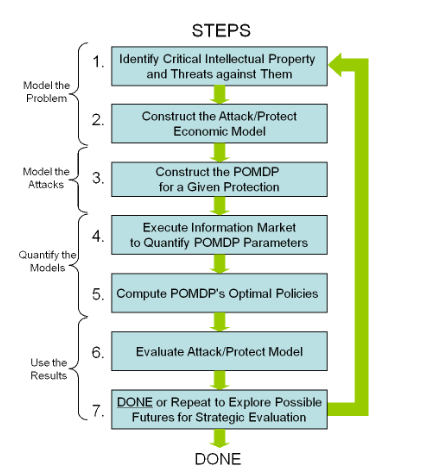
\includegraphics[scale=0.5]{latex/kuvat/queries.png}
    \caption{The QuERIES methodology is used as a reference flowchart for evaluation of security. \cite{hughes2013quantitative}}
    \label{queriesimg}
\end{figure}

\subsection{QuERIES as a central methodology}

QuERIES draws inspiration from computer science, game theory, control theory, and economics, thus is a complex answer to a complex question. It is stated that it can be used as an alternative to popular methodologies such as red teaming or black-hat analysis used commonly in risk-assessment. \cite{carin2008cybersecurity}

QuERIES is proposed to have potentially significant usage in DoD (Department of Defense) and in private sector \cite{carin2008cybersecurity}. Initial testing of QuERIES in small-scale, realistic scenarios presented by Carin et al. suggest that the methodology can in fact be used as to improve risk-assessment more complex settings \cite{carin2008cybersecurity}. This thesis follows similar steps: first the QuERIES methodology is used to assess risks, then they are generalized with strict constraints in mind. 

\subsection{Partially observable Markov decision process}

Lastly, using the results of the POMDP can be used to increase the protection against the discovered problems. As POMDP provides us data on two things: found security breaches and their security implications through the reward function. 

%% tähän backed up by facts settiä?

The models and attacks are quantified through a partially observable Markov decision process (POMDP). A good way of thinking why are all probabilities taken in to account is Murphy's law: "anything that can go wrong, will go wrong". This is the philosophy behind POMDP, which contains these seven steps:
\begin{enumerate}
    \item Define possible states the system can be in
    \item Define the actions the system can take
    \item Define the possible observations the system can take
    \item Define the transition probabilities of the system
    \item Define the observation probabilities of the system
    \item Rewards: guide the system towards the desirable actions and states.
\end{enumerate} \cite{hughes2013quantitative}

A POMDP is used widely in this kind of applications, as both blue and red team have only partial observations related to the system. While the blue team can't be completely certain that the system is secure, the red team cannot perform fully reliably, as systems and environments differ from each other. \cite{mcabeeMarkov}